This section highlights two optimal strategies to discover $\D(\scoma^*)$: a) exhaustive search, which reveals the search space of all possible sequences of object pairs $ \scoma $ and b) an MILP model. Both alternatives, however, suffer from scalability issues as for each possible assignment, it is necessary to solve a coordinated motion planning problem for the arms. This motivates minimizing the number of assignments $\coma$ considered, and the number of motion planning queries it requires for discovering $\D(\scoma^*)$, while still aiming for high quality solutions.

\noindent\textbf{Exhaustive Search}: The exhaustive search approach shown in Fig. \ref{fig:backtracking} is a brute force expansion of all possible sequences of object pairs $ \scoma $. Nodes correspond to transfers $T(\coma_i)$ and edges are moves $M(\coma_{i\rightarrow i{^\prime}})$. The approach evaluates the cost for all possible branches to return the best sequence $\scoma$. The total number of nodes is in the order of $O(n!)$, expressed over the levels $L$ of the search tree as: 
% \kiril{It may be beneficial to explain the formula below, or perhaps move it to the appendix to save space and avoid explaining it here.}:

% \vspace{-0.25in}
\begin{equation*}
{\permu[n]{2}} + {\permu[n]{2}}\times{\permu[n-2]{2}} + ... + {\permu[n]{2}}\times{\permu[n-2]{2}}\times{\permu[n-4]{2}}...\times{\permu[2]{2}} =\sum_{L=1}^{n/2} {\ \prod_{k=0}^{2L-1}{(n-k)}},
% \vspace{-0.15in}
\end{equation*}
where $\permu[n]{k}$ is the $k$-permutations of $n$.  

\begin{wrapfigure}{r}{2.4in}
    % \vspace{-.5in}
	\centering
	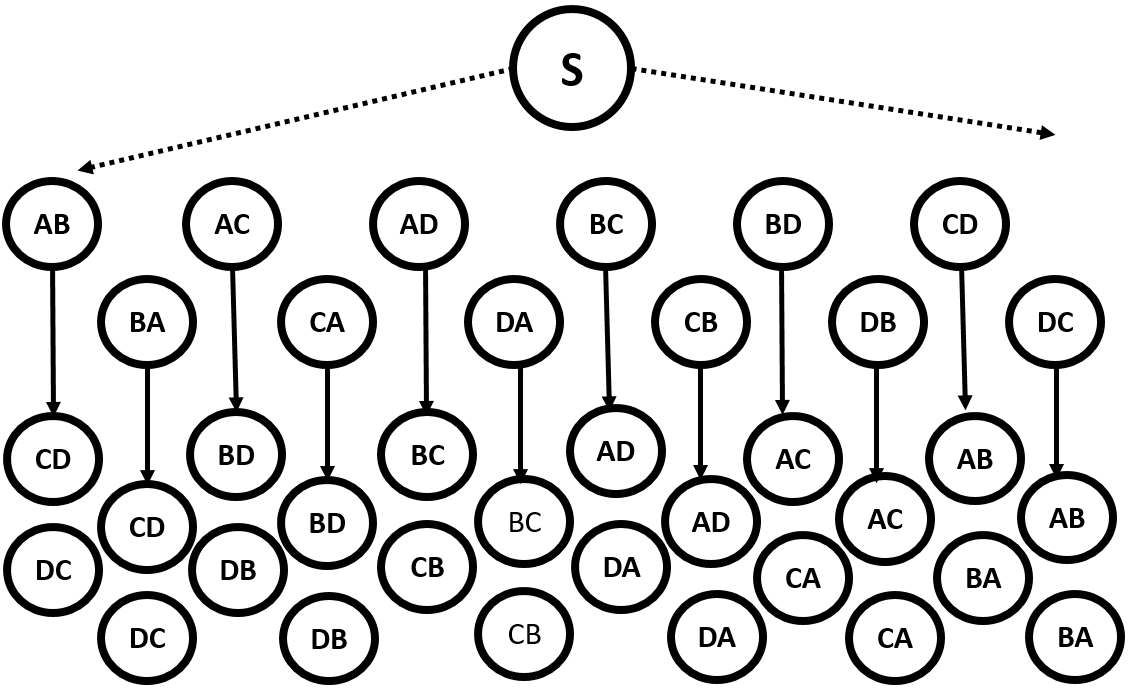
\includegraphics[width=1.8in]{figures/dual_backtracking.PNG}
    % \vspace{-.15in}
	\caption{Search tree for 4 objects. 
%	In node $XY$, $m^1$ transfers object $X$, and $m^2$ transfers $Y$. An edge is a transit to the next node. 
	}
	\label{fig:backtracking}
    % \vspace{-.3in}
\end{wrapfigure}
Motion plans can be reused, however, and repeated occurrences of $T(\coma_i)$ and $M(\coma_{i\rightarrow i^{\prime}})$ should be counted only once for a total of: 
\begin{myitem}
\item[$-$] $  {\permu[n]{2}} $ \textit{transfers} of objects, and 
\item[$-$] $ {{\permu[n]{2}}\times\permu[n-2]{2}} $ \textit{transits} between all possible valid ordered pairs of $ \coma $.
\end{myitem}
Additional motion plans are needed for the initial move from $q_{\rm safe}^k$ and the return to it at the end of the process, introducing $ 2\times\permu[n]{2} $ transits:

% \vspace{-0.25in}
\begin{equation}
\textrm{\# of Transfers} + \textrm{\# of Moves} =  {\permu[n]{2}} +   \Big{(}({{\permu[n]{2}}\times\permu[n-2]{2}}) + (2\times{\permu[n]{2}})\Big{)}
\label{eq:mpcount}
% \vspace{-0.15in}
\end{equation}

This returns optimal synchronized solution but performs an exhaustive search and requires exponentially many calls to a motion planner.

\noindent\textbf{MILP Formulation}:
Mixed Integer Linear Programming (\milp) formulations can utilize highly optimized solvers \cite{gurobi}. Prior work has applied these techniques for solving m-TSP \cite{rathinam2006matroid,friggstad2013multiple} and pickup-and-delivery problems \cite{coltin2014multi,savelsbergh1995general}, but viewed these problems in a decoupled manner. This work outlines an \milp formulation for the synchronized dual-arm rearrangement problem that reasons about coordination costs arising from arm interactions in a shared workspace.

\textit{Graph Representation:}
The problem can be represented as a directed graph where each vertex $v = \coma_v = (\object_v^1, \object_v^2)$ corresponds to a transfer $ T(\coma_u) $ and edges $e(u,v)$ are valid moves $M(\coma_{u\rightarrow v})$. A valid edge $e(u,v)$ is one where an object does not appear more than once in the transfers of nodes $u$ and $v$.  The cost of a directed edge $e(u,v)$ encodes both the cost of the transfer  $ T(\coma_v) $ and the cost of the move $M(\coma_{u\rightarrow v})$. There is also a vertex $ \startq $, which connects moves from and to the safe arm configurations $q^k_{\rm safe}$.  The directed graph $ \hat{G} (\hat{V},\hat{E}) $ is defined:

% \vspace{-.25in}
\begin{align*}
\hspace{0.5in} \hat{V} = \{ v = \coma_v = (\object_v^1,\object_v^2)\ | \  \forall\ \object_v^1,\object_v^2 \in \objectset, \object_v^1 \neq \object_v^2 \} \cup \{S\}\\
\hat{E} = \{  e(u,v)\ | \ \forall\ u,v\in \hat{V} \textrm{ so that } u\neq v,\ \object_v^k \neq \object_u^{\ell}\ \forall\ k, \ell \in [1,2] \}\\
\cup\ \{e(\startq,v)\ \forall\ v\in\hat{V}\setminus \startq\} \cup \{e(v,\startq)\ \forall\ v\in\hat{V}\setminus \startq\}\\
cost_{e(u,v)} = \cost(u) + \cost(u,v) =\cost(T(\coma_u)) + \cost(M(\coma_{u\rightarrow v}))
\end{align*}

% \vspace{-.15in}
Let $\cost(\startq) = 0$. The total number of motion planning queries needed to be answered to define the edge costs is expressed in Eq.~\ref{eq:mpcount}. The formulation proposed in this section tries to ensure the discovery of $ \scoma^* $ on $ \hat{G} $ as a tour that starts and ends at $ \startq $, while traversing each vertex corresponding to $ \scoma^* $. To provide the {\tt MILP} formulation, define $ \delta_{\rm in}(v) $ as the in-edge set $v$, and  $ \delta_{\rm out}(v) $ as the out-edge set. Then, $ \gamma(\object) $ is the object coverage set $ \gamma(\object) = \{ e(u,v) \ |\ e\in\hat{E}, \object\in  \coma_u  \} $, i.e., all the edges that transfer $ \object $.

\textit{Model:} Set the optimization objective as: $\ \ \min \sum_{e \in \hat{E}} cost_e x_e\  $\hspace{.81in} [A]\\ 
Eq. [B] below defines indicator variables. Eqs. [C-E] ensure edge-flow conserved tours. Eqs. [F-G] force $\startq$ to be part of the tour. Eq. [H] transfers every object only once. Eq. [I] lazily enforces the tour to be of length $ \frac{n}{2} + 1 $. While the number of motion-planning queries to be solved is the same as in exhaustive search, efficient {\milp} solvers \cite{gurobi} provide a more scalable search process.

% \vspace{-.2in}
\noindent\begin{minipage}{.5\textwidth}
\begin{align*}
x_e \in \{ 0,1 \}& \ \ \forall e \in \hat{E} \tag*{[B]}\\
\sum_{e\in\delta_{\rm in}(v)} x_e \leq 1& \ \ \forall v\in \hat{V} \tag*{[C]}\\
\sum_{e\in\delta_{\rm out}(v)} x_e \leq 1& \ \ \forall v\in \hat{V} \tag*{[D]}\\
\sum_{e\in\delta_{\rm in}(v)}x_e = \sum_{e\in\delta_{\rm out}(v)}x_e& \ \ \forall v\in \hat{V} \tag*{[E]}\\
\end{align*}
\end{minipage}
\noindent\begin{minipage}{.5\textwidth}
\begin{align*}
\sum_{e\in\delta_{\rm in}(\startq)} x_e = 1& \tag*{[F]}\\
\sum_{e\in\delta_{\rm out}(\startq)} x_e = 1& \tag*{[G]}\\
\sum_{e\in\gamma(\object)} x_e = 1& \ \  \forall \object\in\objectset \tag*{[H]}\\
\sum_{e(u,v)\in \mathfrak{T}} x_e < |\mathfrak{T}| & \ \  \forall \mathfrak{T} \subset \hat{V}, |\mathfrak{T}| \leq \frac{n}{2} \tag*{[I]}
\label{model:milp}
\end{align*}
\end{minipage}

